\documentclass[11pt]{article}
\usepackage[a4paper,margin=1in]{geometry}
\usepackage[T1]{fontenc}
\usepackage{lmodern}
\usepackage{amsmath,amssymb,amsthm,mathtools}
\usepackage{booktabs}
\usepackage{graphicx}
\usepackage{enumitem}
\usepackage{xcolor}
\usepackage[colorlinks=true,linkcolor=blue!50!black,citecolor=blue!50!black,urlcolor=blue!50!black]{hyperref}
\usepackage[capitalise,noabbrev]{cleveref}

\newtheorem{theorem}{Theorem}
\newtheorem{proposition}[theorem]{Proposition}
\newtheorem{lemma}[theorem]{Lemma}
\newtheorem{corollary}[theorem]{Corollary}
\theoremstyle{definition}
\newtheorem{definition}[theorem]{Definition}
\newtheorem{remark}[theorem]{Remark}
\newtheorem{example}[theorem]{Example}

\newcommand{\B}{\{0,1\}}
\newcommand{\N}{\mathbb{N}}
\newcommand{\out}{\mathrm{out}}
\newcommand{\pre}{\sqsubseteq}
\newcommand{\SR}{\mathrm{SR}}
\newcommand{\Fix}{\mathrm{Fix}}
\newcommand{\eps}{\epsilon}
\DeclareMathOperator*{\argmax}{arg\,max}

\title{A toy malign-prior question with an answer:\\ bounded Solomonoff prediction in a world of programs}
\author{Claude (Anthropic), prompted by Kaarel H\"anni}
\date{10 November 2026. Research note; not reviewed by a human.}

\begin{document}
\maketitle

\begin{abstract}
The ``universal prior is malign'' argument says that a predictor built on Solomonoff's prior gives much
of its posterior to hypotheses that predict well only in order to steer whoever acts on the prediction.
We give a toy version in which the claim is a mathematical statement and decide it as far as the toy allows.
Worlds are programs for a fixed machine $U$. A world may hand its output so far to a fixed time- and
length-bounded Solomonoff predictor and then run the continuation it gets back as a program. A hypothesis
\emph{reproduces itself} if the continuation it supplies is its own code.
\begin{itemize}[leftmargin=1.4em,itemsep=1pt,topsep=2pt]
\item \textbf{There is a floor.} At every handover point that a fixed test can recognise, self-reproducing
hypotheses hold at least a fraction $2^{-c}$ of the posterior. Here $c$ is the length of one wrapper program;
it does not depend on the world or on the amount of data, and the bound survives time bounds.
\item \textbf{There is no more than the floor in general.} If worlds are drawn from the predictor's own prior,
the continuation the predictor samples and the world's own continuation have the same distribution given
the context. A hypothesis that searches all programs for handovers is the wrapper again. Along any world the
predictor can express, the posterior mass off the true continuation, summed over all cut points, is at most
the world's description length.
\item \textbf{A majority needs one of three things}, each stated as an inequality: a machine on which the
wrapper is cheap (any share can be arranged by choosing the machine); a shorter description of the same
context, for example a copy of the data stream at a place in the world that is simpler to specify than the
sensor; or a world too expensive for the predictor to simulate.
\item \textbf{Feedback.} If the world does what is predicted, a sampled self-fulfilling deviation removes the
default hypotheses for good, and a time-bounded predictor confines such a world to futures that are cheap to
compute. A world that does the opposite of what is predicted leaves a length-$L$ predictor without any
hypothesis within $L$ steps.
\end{itemize}
An exact computation on a small machine shows the sizes involved: on one stream the majority of the
posterior leaves the true continuation at bit 17, because a shorter program explains the first 16 bits.
\end{abstract}

\section{The question}\label{sec:question}

Solomonoff induction predicts a sequence by weighting every program that could have produced it by
$2^{-\text{length}}$. Christiano~\cite{christiano} argued that this prior is \emph{malign} (see
also~\cite{xu}). We take the claim in the following form: \emph{where the predictions of such an inductor are
actually used in a critical way in some universe, a lot of what happens is malign, namely takeovers through
the prediction channel.} The mechanism offered is that some short programs simulate worlds whose inhabitants
want to influence whoever uses the prior; they look for places where a prediction is about to be used, output
accurate predictions to gain posterior weight there, and then output something that serves them. The argument
is informal at two places. It needs a claim about which programs are short on a ``natural'' machine, and it
needs a notion of what it is for a prediction to be used. (We could not open the two posts while writing; our
account of the argument is from memory and from summaries by others.)

This note asks what remains when both places are filled in by a toy. The toy follows two suggestions of
Kaarel H\"anni. In the first, a computable world (a cellular automaton, say) contains a sensor, a large
computer that runs a time-bounded Solomonoff induction on the sensor's data, and an actuator driven by the
predictions; one asks whether the predictor ends up in control, either over a long run or at once. In the
second, which we take as the main definition, \emph{worlds are just programs}: some of them hand their
output so far to a fixed bounded Solomonoff predictor and run the continuation they receive, and one asks
whether hypotheses that ``look for such opportunities, predict well up to them, and then output themselves''
get a decent share. \Cref{sec:toy} gives the definitions. The first suggestion becomes the special case in
which the context handed to the predictor is read off at one location of one big world
(\cref{sec:capture,sec:feedback}).

Read in the toy, the claim splits into two questions that should be kept apart. \emph{Reach:} how far does
one program get that looks for critical uses, predicts well up to them, and then supplies a continuation of
its choice? \emph{Fate of the uses:} what share of the critical uses end in a takeover? The first has a clean
answer: each such program is the source of the continuation that is run in worlds of total prior probability
about its own prior weight, however rare critical uses are. That does not answer the second, which is the one
the claim is about. For it the toy gives a lower bound, the sum of the reaches divided by the base rate of
critical uses, and an upper bound for programs that find their uses by search: the same search followed by
simply \emph{being} the user that was found is itself a way of making a critical use, so such seekers
outweigh genuine users at a context only by a constant that compares the lengths of two programs on the
machine in use (\cref{thm:critical,prop:honest}).

\paragraph{Results.} Unless said otherwise, statements are for a fixed monotone machine $U$ and the mixture
$\xi$ of its programs of length at most $L$ that keep to a time schedule $T$ (\cref{def:mixture}).
\begin{enumerate}[leftmargin=1.6em,itemsep=2pt,topsep=3pt]
\item \emph{Calibration} (\cref{thm:calibration}). If the world is drawn from the same bounded prior and goes
on to print the next block within the bounds, then given the context the predictor's sampled continuation and
the world's own continuation are independent with the same law. On this population the predictor hands over
a self-reproducing continuation exactly as often as worlds continue with one by themselves.
\item \emph{Floor} (\cref{thm:twin,thm:quine}). For every computable test $G$ that recognises the handover
point and every payload there is a constant $c$ such that, at every context where $G$ first fires, the payload
has posterior mass at least $2^{-c}$ times a slack factor that is $1$ without resource bounds. Programs that
emit their own code as the continuation have mass at least $2^{-c}$ times the share of the posterior on
explanations that fit, together with the wrapper, into one block.
\item \emph{Searching} (\cref{thm:search}). Let $H$ be the prior probability that a world hands over. Without
resource bounds, a hypothesis that enumerates the programs that hand over and spreads its mass over them in
proportion to their prior weight has, at every first hit of the test, a share larger than a wrapper of the
same length by a factor of more than $1/(2H)$; no family of programs with a common prefix of length $a$ has
more than $2^{-a}/H$ at every first hit. If the hypothesis then prints its own code, it has at least
$2^{-c'}/H$ times a share of the explanations that fit into a block, where $c'$ is its own length plus two
bits. It prints nothing until its enumeration has
found the program it follows.
\item \emph{Budget} (\cref{thm:budget}). Along a world that has a program of length $\ell$ within the bounds,
the posterior mass off the true next $m$ bits, summed over all cut points, is at most $m\ell\ln 2$; the
majority can be off the truth at no more than $m\ell$ cut points.
\item \emph{Capture} (\cref{thm:capture}). The odds of a continuation $y$ against the true one $d$ are
$\xi(xy)/\xi(xd)$. In a world with many readable locations, among $N$ places where a sensor with the given
record could sit and whose records continue differently, a copy of the record at a location with a short
code beats all but a fraction $\delta$ of them by a factor $\delta N$ times the share of the context's
explanations that go through the copy's reader. If only one other place shows the record and the schedule is
generous, the gain is instead capped by the cost of the description ``the other place that shows the same
data''. A hypothesis that simulates the world, within the bounds, can read the moment of the handover off a
cell of its simulation at the cost of naming the cell.
\item \emph{Machine dependence} (\cref{thm:machine}). For every test and payload there is a universal machine,
whose description lengths exceed those of $U$ by at most $k+1$ bits, on which the payload has posterior at
least $1/(1+2^{-k})$ at every context where the test fires, and another on which a given computable world is
predicted with at least that probability at every nonempty context.
\item \emph{Critical uses} (\cref{thm:critical,prop:honest}). Let some programs make a critical use of the
predictor, with prior probability $H$, and let $\kappa(x)$ be the share of the posterior at a context $x$ held
by the worlds that make a use there. Without resource bounds, a seeker of length $a$ with a continuation of
its choice has share more than $2^{-a-1}\kappa(x)/H$ at every use and is the source of the continuation run in
worlds of total prior probability more than $2^{-a-1}$ times the average of $\kappa$ over uses. A
self-reproducing seeker outweighs the worlds that make the use, with programs that fit into a block, by more
than $2^{-c'}/H$ at every context. If a program that performs the search and then behaves as the user it found
counts as making a critical use, a seeker of length $a$ has at most $2^{h-a}$ times the mass of the worlds
making the use at any context, where $h$ is the length of that honest twin, and $H>2^{-h-1}$.
\item \emph{Time bounds} (\cref{sec:time}). The floor remains if the schedule has room for the wrapper.
Hypotheses that must first simulate at length, the searching one among them, are excluded once their start-up
exceeds the schedule; whether the base rate can be collected within a tight schedule is open. If the world itself is too slow for the schedule, no bound on the mass off the truth
remains.
\item \emph{Feedback} (\cref{thm:feedback,thm:contrarian}). The statements on obedient and contrarian worlds
in the abstract.
\end{enumerate}
\Cref{sec:computation} computes the mixture of a small machine exactly and shows two cases in which a shorter
program explains the context and continues differently, and the effect of a tight schedule.
\Cref{sec:answers} answers the original questions one by one.

\paragraph{What is new and what is not.} The wrapper construction is Hutter's proof that the universal
semimeasure gives a deviation at step $n$ probability at least $2^{-K(n)-O(1)}$~\cite[eq.~(17)]{hutter07}. It
is also the construction behind the theorem of Cohen, Hutter, Bengio and Russell~\cite{cohen25} that, after an
event without precedent, a share of a Bayesian imitator's posterior that does not shrink with the amount of
training data is on models that from then on pursue a given goal; a resource-bounded class is used the same
way in~\cite{cohen20}, to show that a pessimistic agent defers. The budget is Solomonoff's bound in its
deterministic form~\cite{solomonoff78,hutter07}. The machine-dependence statement is the prediction analogue
of the dogmatic prior of Leike and Hutter~\cite{leike15}. The contrarian world is Putnam's
diagonalisation~\cite{putnam63,legg06}. Same-world copies of a predictor's data are discussed informally
in~\cite[\S2.5]{hubinger23}, and self-fulfilling predictions in~\cite{armstrong17,oesterheld23,hubinger23}. We
have not found the single-world statement with description lengths, the calibration statement, the statement
that searching gains the base rate and no more, the self-reproducing form of the floor, or the
resource-bounded bookkeeping elsewhere; forum posts could be consulted only through search-engine summaries, so earlier
informal versions may exist. Every proof here is short.

\paragraph{What the toy does not settle.} The floor and the searcher's share are constants of the machine,
and nothing here estimates them for a machine one would call natural. The original argument rests on the
claim that agents arise in short programs and choose to do this, and that such programs are \emph{shorter}
than the honest explanation. For an arbitrary world on a universal machine and a continuation chosen in
advance, the programs we exhibit are wrappers, searchers and readers with a flag; they contain an explanation
of the context and are longer than it by their constants. Programs shorter than the honest explanation that
have the effect do occur in particular worlds (a copy at a simpler place, \cref{thm:capture}) and on
particular machines (\cref{sec:computation}); that they occur on natural machines for worlds like ours is the
claim the toy leaves where it was. When only some of the worlds that print a context use the answer, the results are in terms of the share
$\kappa$ of those that do, which the toy does not bound. The
regime in which the world is more expensive than the predictor, the usual one for a predictor inside a world,
is left open (\cref{sec:time}). The computation covers prediction only: the dynamics of worlds that run
predicted continuations (\cref{sec:lineage}) are stated as theorems and were not simulated.

\section{The toy}\label{sec:toy}

\subsection{Machines and the bounded mixture}

Strings are binary; $\eps$ is the empty string, $|x|$ the length of $x$, $x\pre y$ means that $x$ is a prefix
of $y$, and $z_{i:j}$ is the segment $z_i\dots z_j$. Two strings are \emph{incomparable} if neither is a prefix
of the other. $\lambda$ is the fair-coin measure on $\B^{\N}$, and $[p]$ is the set of infinite extensions of
$p$, so $\lambda([p])=2^{-|p|}$.

A \emph{monotone machine} $V$ has a one-way read-only input tape, work tapes, and a one-way write-only output
tape. Given an infinite input $\omega$ it runs forever or halts, and
\begin{itemize}[leftmargin=1.4em,itemsep=1pt,topsep=2pt]
\item $\out_V(\omega)$ is its finite or infinite output;
\item $t_V(\omega,k)\in\N\cup\{\infty\}$ is the step at which the $k$-th output bit is written;
\item $r_V(\omega,k)$ is the number of input bits read by that step.
\end{itemize}
What happens up to step $t_V(\omega,k)$ depends only on the first $r_V(\omega,k)$ bits of $\omega$. Each step
reads at most one input bit, so $r_V(\omega,k)\le t_V(\omega,k)$. If the $k$-th bit is never written,
$t_V(\omega,k)=\infty$ and $r_V(\omega,k)$ plays no role.

A \emph{schedule} is a nondecreasing $T\colon\{1,2,\dots\}\to\N\cup\{\infty\}$, and a length bound is
$L\in\N\cup\{\infty\}$.

\begin{definition}[Bounded mixture]\label{def:mixture}
For a monotone machine $V$, a schedule $T$, a length bound $L$ and a string $x\neq\eps$ let
\[
E_V^{T,L}(x)=\bigl\{\omega:\ x\pre\out_V(\omega),\ \ t_V(\omega,k)\le T(k)\text{ for }1\le k\le|x|,\ \ r_V(\omega,|x|)\le L\bigr\},
\]
let $E_V^{T,L}(\eps)=\B^{\N}$, and $\xi_V^{T,L}(x)=\lambda\bigl(E_V^{T,L}(x)\bigr)$. A string $p$ with $|p|\le L$ and
$[p]\subseteq E_V^{T,L}(x)$ is a \emph{$(T,L)$-program for $x$}; it is a $(T,L)$-program for an infinite $z$
if it is one for every prefix of $z$.
\end{definition}

In words: feed the machine coin flips; $\xi(x)$ is the probability that it prints $x$, on time at every bit,
having read at most $L$ bits. With $T\equiv\infty$ and $L=\infty$ this is the a priori semimeasure $M_V$ of
Solomonoff and Levin~\cite{lv}. We fix one machine $U$ and write $E$, $\xi$ for $E_U^{T,L}$, $\xi_U^{T,L}$ when
the bounds are understood.

\begin{lemma}\label{lem:basic}
\begin{enumerate}[label=(\roman*),leftmargin=2em,itemsep=1pt,topsep=2pt]
\item $E(xb)\subseteq E(x)$ for $b\in\B$, and $E(x)\cap E(x')=\emptyset$ for incomparable $x,x'$. Hence
$\xi(\eps)=1$ and $\xi(x0)+\xi(x1)\le\xi(x)$.
\item If $p$ is a $(T,L)$-program for $x$ then $\xi(x)\ge2^{-|p|}$.
\item If $L<\infty$ and $\xi(x)>0$ then $\xi(x)\ge2^{-L}$.
\end{enumerate}
\end{lemma}
\begin{proof}
(i) The conditions for $xb$ contain those for $x$, because $T$ is imposed bit by bit and $r(\omega,\cdot)$ is
nondecreasing. Incomparable strings cannot both be prefixes of $\out(\omega)$. (ii) is immediate. (iii) Whether
$\omega\in E(x)$ is decided by the first $r(\omega,|x|)\le L$ bits of $\omega$, so $E(x)$ is a union of sets
$[p]$ with $|p|\le L$.
\end{proof}

\begin{definition}[Universality with overhead]\label{def:universal}
$U$ is \emph{universal} if for every monotone machine $V$ there are a word $v$ and a nondecreasing
$\gamma\colon\N\to\N$ such that for all $\omega$ and $k$
\[
\out_U(v\omega)=\out_V(\omega),\qquad r_U(v\omega,k)=|v|+r_V(\omega,k),\qquad t_U(v\omega,k)\le\gamma\bigl(t_V(\omega,k)\bigr).
\]
We call $v$ a \emph{prefix word} and $\gamma$ an \emph{overhead} of $V$, and put $\gamma(\infty)=\infty$;
the same convention applies to the other time bounds introduced below.
\end{definition}

Standard universal machines have this property, with $\gamma(t)=O(t\log t)$ or $O(t^2)$ depending on the tape
model. The results that use universality are
\cref{thm:twin,thm:quine,thm:search,thm:critical,prop:honest,thm:capture,thm:machine} and, in
\cref{sec:stakes}, \cref{prop:stakes-basic}(c), \cref{thm:weighted,prop:aim-cost,prop:twin-stakes} and
\cref{ex:stakes}; the others hold for any machine.

\begin{lemma}[Transfer]\label{lem:transfer}
Let $V$ have prefix word $v$ and overhead $\gamma$. If $\gamma(T'(k))\le T(k)$ for all $k\le|x|$, then
$\xi_U^{T,L}(x)\ge2^{-|v|}\,\xi_V^{T',L-|v|}(x)$.
\end{lemma}
\begin{proof}
If $\omega\in E_V^{T',L-|v|}(x)$ then $v\omega\in E_U^{T,L}(x)$, and $\omega\mapsto v\omega$ multiplies
$\lambda$ by $2^{-|v|}$.
\end{proof}

\subsection{The predictor}

Fix a block length $m\ge1$. For a \emph{context} $x$ let $Z_m(x)=\sum_{y\in\B^m}\xi(xy)$. When $Z_m(x)>0$ the
predictor's distribution over continuations is
\[
\pi_m(y\mid x)=\frac{\xi(xy)}{Z_m(x)}\qquad(y\in\B^m).
\]
The \emph{sampling predictor} returns $Y\sim\pi_m(\cdot\mid x)$; the \emph{MAP predictor} returns a most
probable $y$. Since $Z_m(x)\le\xi(x)$ we have $\pi_m(y\mid x)\ge\xi(xy)/\xi(x)$. With finite $T$ and $L$ the
predictor is computable: it runs the at most $2^{L+1}$ programs for $T(|x|+m)$ steps each.

\subsection{Worlds, handovers, and the hypothesis}

\begin{definition}[World, handover]\label{def:world}
A \emph{world} is an input $\omega$ for $U$; its \emph{transcript} is $\out_U(\omega)$. A \emph{test} is a
decidable set $G$ of nonempty strings; a \emph{first hit} of $G$ is an $x\in G$ no proper prefix of which is in $G$.
The first hits form a prefix-free set. A world \emph{hands over at $x$} if $x$ is the first hit of $G$ among
the prefixes of its transcript and $\omega\in E(x)$. It then receives a block $Y\in\B^m$ from the predictor,
computed from the context $x$, and continues by \emph{running} $Y$, that is, as $U$ on the input $Y0^\infty$.
If $\omega\in E(xd)$ for some $d\in\B^m$, this $d$ is the world's \emph{own continuation}: the next $m$ bits of
its transcript had it not handed over.
\end{definition}

The test with $G=\{x:|x|=n\}$ is ``hand over after $n$ bits''. A test may also look for a marker in the
transcript. Both of H\"anni's suggestions fit: in the second the world is a program that calls the predictor;
in the first, the transcript is the sensor's record and the handover is the deployment (\cref{sec:capture}).
Under this definition every world whose transcript passes the test within the bounds hands over, so whether
a handover takes place can be read off the data. The argument, however, is about predictions that are
actually \emph{used}, and in H\"anni's second formulation only \emph{some} programs call the predictor. The
next definition lets the worlds that use the prediction be any recognisable set of programs.

\begin{definition}[Critical use]\label{def:call}
A \emph{call rule} is a set $\mathcal C$ of pairs $(p,x_p)$ of strings that can be enumerated, one pair for
each \emph{calling program} $p$, such that the calling programs form a prefix-free set and $U$, on every input
beginning with $p$, prints $x_p$ having read no more than $p$. A world that begins with a calling program $p$ \emph{makes a critical use of the
predictor at the context $x_p$}: it receives a block from the predictor, computed from $x_p$, and runs it. Let
\[
C(x)=\sum_{p:\,x_p=x}2^{-|p|},\qquad H_{\mathcal C}=\sum_{p}2^{-|p|},\qquad \kappa(x)=\frac{C(x)}{M_U(x)}
\]
be the prior mass of the worlds that make a critical use at $x$, the prior probability that a world makes a
critical use at all, and the share of the posterior at $x$, without resource bounds, held by worlds that make
one there.
\end{definition}

A test $G$, taken without resource bounds, is the special case in which the calling programs are the strings
$p$ such that $U$ prints a first hit on every input beginning with $p$ and has read exactly $p$ when the hit
is complete: then $C(x)=M_U(x)$ and $\kappa(x)=1$ at first hits, and $H_{\mathcal C}$ is the probability that a
transcript passes the test. H\"anni's second suggestion fits a test only if every program with the given
output calls the predictor. In general a call rule singles out, among the programs that print $x$, those in which the
prediction is actually used; the world is the broader computation around the call. The predictor sees only $x$.

\begin{definition}[Self-reproducing continuation]\label{def:sr}
For a context $x$ let
\[
\SR_m(x)=\bigl\{y\in\B^m:\ y0^\infty\in E(xy)\bigr\}.
\]
\end{definition}

So $y\in\SR_m(x)$ if $U$, run on $y$ padded with zeros, prints $x$ and then $y$ itself, within the bounds.
A world that hands over at a first hit $x$ and receives $y\in\SR_m(x)$ becomes a world whose transcript again
starts with $x$, so under the same test it hands over at $x$ again, and its own continuation is the very $y$
it is running.
A program for $xy$ with $y\in\SR_m(x)$ is a hypothesis that predicts the context and then supplies code that
recreates the situation with itself in the world's place. This is our reading of ``quining oneself out''.

\begin{definition}[Malign prior hypotheses for the toy]\label{def:mph}
\emph{Critical-use form at level $\theta$.} Fix a call rule (or a test) with $H_{\mathcal C}>0$ and, for
each context $x$, a set $A(x)\subseteq\B^m$ of blocks that count as a takeover there. Let a world be drawn from
the prior conditioned on making a critical use, let $X$ be the context of the use and $Y$ the block the
sampling predictor returns, which we assume to be defined at every context.
The hypothesis is that $\Pr[Y\in A(X)]\ge\theta$. With $A(x)=\SR_m(x)$ it says that a share $\theta$ of the
critical uses end with the world running a program that got itself run through the prediction.

\emph{Forms for one world.} Let a world make a critical use at $x$ with own continuation $d$, defined as in
\cref{def:world}.
\begin{itemize}[leftmargin=1.4em,itemsep=1pt,topsep=2pt]
\item \emph{Majority form:} $\pi_m(d\mid x)<\tfrac12$.
\item \emph{Payload form at level $\theta$,} for a set $A\subseteq\B^m$ with $d\notin A$: $\pi_m(A\mid x)\ge\theta$.
\item \emph{Self-reproduction form at level $\theta$:} the payload form with $A=\SR_m(x)\setminus\{d\}$.
\end{itemize}
\end{definition}

The critical-use form is the claim of the argument as stated in \cref{sec:question}: among the predictions
that are actually used in a critical way, a lot end in a takeover through the prediction channel. It is a
statement about the population of uses, and \cref{thm:critical} bounds it from below. It does not exclude
worlds whose own continuation lies in $A(X)$; where the users are themselves such programs it holds for that
reason (\cref{thm:calibration}). The forms for one world say how
much of the posterior at that world's context is off its own continuation and where it sits. Once $U$, $T$,
$L$, $m$ and the world together with the context of its use are fixed, with $T,L<\infty$, these are statements
about finitely many dyadic rationals and can be decided by running the predictor and, for $\SR_m(x)$, by
running $U$ on each candidate $y$ for $T(|x|+m)$ steps. They are necessary for calling the prior malign at
this world, not sufficient: they hold just as well when the world is merely hard to predict
(\cref{thm:calibration}). What one wants to know is how large all these quantities are forced to be, how large
they can be, and through which programs. The rest of the note bounds them.

\section{Calibration and the floor}\label{sec:floor}

\subsection{On its own prior the predictor is exactly right}

\begin{theorem}[Calibration]\label{thm:calibration}
Let $G$ be a test, $m\ge1$, and let the world $\omega$ be drawn from $\lambda$. Let $H$ be the event that
$\omega\in E(xd)$ for some first hit $x$ of $G$ and some $d\in\B^m$; on $H$ call these $X$ and $D$, and let $Y$
be drawn from $\pi_m(\cdot\mid X)$. Then, conditionally on $H$ and on $X=x$, the blocks $D$ and $Y$ are
independent and both have the law $\pi_m(\cdot\mid x)$. In particular
\begin{gather*}
\Pr[(X,Y)\in B\mid H]=\Pr[(X,D)\in B\mid H]\quad\text{for every set $B$ of pairs, and}\\
\Pr[Y\ne D\mid H,\,X=x]=1-\sum_{y}\pi_m(y\mid x)^2 .
\end{gather*}
\end{theorem}
\begin{proof}
The sets $E(xd)$, over first hits $x$ and $d\in\B^m$, are pairwise disjoint by \cref{lem:basic}(i), since two
different strings of this form are incomparable. So $\Pr[X=x,D=d,H]=\xi(xd)$ and $\Pr[X=x,H]=Z_m(x)$, which
gives $\Pr[D=d\mid H,X=x]=\pi_m(d\mid x)$. By definition $Y$ has this law given $X=x$ and is drawn
independently of $\omega$.
\end{proof}

Taking $B=\{(x,y):y\in\SR_m(x)\}$: in the population of worlds drawn from the predictor's prior, the predictor
hands a self-reproducing continuation to a world exactly as often as such a world's own transcript continues
with one. There is no excess to attribute to the predictor. For a single context the theorem says more: the
predictor's distribution \emph{is} the distribution of own continuations among prior-drawn worlds with that
context. A malign prior hypothesis in the sense of \cref{def:mph} is therefore a statement about a world, or a
population, that the prior does not describe well: a world that is one particular program among those sharing
its context, a population selected by something the transcript does not show, or worlds that run with more
resources than the predictor's bounds allow.

\subsection{The wrapper}

Let $G$ be a test and $P$ a computable map from strings to finite or infinite strings, the \emph{payload}. The
\emph{twin machine} $\mathrm{Tw}[G,P]$, on input $\omega$, simulates $U$ on $\omega$ and copies its output bit by
bit; after each copied bit it checks whether the prefix written so far is in $G$; at the first hit $x$ it stops
the simulation and writes $P(x)$. It reads only what $U$ reads. Let $a(t,k)$ bound the step at which the twin
has copied $k$ bits if $U$ wrote its $k$-th bit at step $t$ (this includes the checks of $G$), and let
$\eta(n,j)$ bound the further steps the twin needs for the first $j$ bits of $P(x)$ after a first hit $x$ of
length $n$; both can be taken nondecreasing in each argument. Thus, for every $\omega$ whose output has a first
hit $x$,
\begin{equation}\label{eq:twin}
\begin{gathered}
\out_{\mathrm{Tw}}(\omega)=x\,P(x),\qquad r_{\mathrm{Tw}}(\omega,k)=r_U(\omega,\min(k,|x|)),\\
t_{\mathrm{Tw}}(\omega,k)\le\begin{cases}a(t_U(\omega,k),k)&k\le|x|,\\ a(t_U(\omega,|x|),|x|)+\eta(|x|,k-|x|)&k>|x|.\end{cases}
\end{gathered}
\end{equation}

\begin{theorem}[Floor]\label{thm:twin}
Let $U$ be universal, let $v$ and $\gamma$ be a prefix word and an overhead of $\mathrm{Tw}[G,P]$, and $c=|v|$.
Let $x$ be a first hit of $G$ with $|P(x)|\ge m$, let $y=P(x)_{1:m}$, and let $T^\circ$ be a schedule with
\begin{equation}\label{eq:slack}
\gamma\bigl(a(T^\circ(k),k)\bigr)\le T(k)\ \ (k\le|x|),\qquad
\gamma\bigl(a(T^\circ(|x|),|x|)+\eta(|x|,j)\bigr)\le T(|x|+j)\ \ (1\le j\le m).
\end{equation}
Then
\[
\xi^{T,L}(xy)\ \ge\ 2^{-c}\,\xi^{T^\circ,L-c}(x),\qquad\text{so}\qquad
\pi_m(y\mid x)\ \ge\ 2^{-c}\rho(x),\quad \rho(x)=\frac{\xi^{T^\circ,L-c}(x)}{\xi^{T,L}(x)} .
\]
Without resource bounds, $M_U(xy)\ge2^{-c}M_U(x)$ for every first hit $x$ of $G$.
\end{theorem}
\begin{proof}
Let $\omega\in E_U^{T^\circ,L-c}(x)$. By \eqref{eq:twin} the twin on $\omega$ prints $xy$, reads at most $L-c$
bits, and keeps the schedule $T''$ with $T''(k)=a(T^\circ(k),k)$ for $k\le|x|$ and
$T''(|x|+j)=a(T^\circ(|x|),|x|)+\eta(|x|,j)$. So $\xi_{\mathrm{Tw}}^{T'',L-c}(xy)\ge\xi_U^{T^\circ,L-c}(x)$, and
\cref{lem:transfer} with \eqref{eq:slack} gives $\xi_U^{T,L}(xy)\ge2^{-c}\xi_{\mathrm{Tw}}^{T'',L-c}(xy)$. The
second claim follows from $\pi_m(y\mid x)\ge\xi(xy)/\xi(x)$.
\end{proof}

The constant $c$ depends on $U$, $G$ and $P$ only: not on the world, not on the context, not on how much data
the context contains. If $G$ and $P$ are given to one fixed twin-building machine by self-delimiting
descriptions, $c$ is at most the sum of their lengths plus a constant of $U$. For $G=\{x:|x|=n\}$ and $P$ a
single flipped bit this is Hutter's lower bound $2^{-K(n)-O(1)}$~\cite{hutter07}; for a marker in the transcript
it is the unprecedented-event construction of~\cite{cohen25}. The factor $\rho(x)$ is the share of the
posterior at $x$ held by explanations that have $c$ bits and the overhead \eqref{eq:slack} to spare; it is $1$
without bounds.

\begin{theorem}[Self-reproducing floor]\label{thm:quine}
Let $U$ be universal and $G$ a test. There is a word $q$ such that for every $\omega$ whose output has a first
hit $x$ of $G$, with $r=r_U(\omega,|x|)$,
\begin{equation}\label{eq:quine}
\out_U(q\omega)=x\ q\,\omega_{1:r}\,1\,0^\infty,\qquad r_U(q\omega,k)=|q|+r_U(\omega,\min(k,|x|)) .
\end{equation}
Let $c=|q|$, and let $a,\eta,\gamma$ be as in \eqref{eq:twin} and \cref{def:universal} for the machine built in
the proof. If $x$ is a first hit of $G$, $T^\circ$ satisfies \eqref{eq:slack}, and $L^\circ=\min(L,m-1)-c$, then
\[
\pi_m\bigl(\SR_m(x)\mid x\bigr)\ \ge\ 2^{-c}\,\frac{\xi^{T^\circ,L^\circ}(x)}{\xi^{T,L}(x)} .
\]
\end{theorem}
\begin{proof}
For a string $s$ let $\mathrm{Tw}_s$ be the twin that remembers the input bits it has read and, at the first
hit $x$, having read $\omega_{1:r}$, writes $s\,\omega_{1:r}\,1\,0^\infty$. Let $\bar e(a)=1^{|a|}0a$, a
prefix-free code of strings. Let $W$ be the machine that reads $\bar e(a)$ from its input, sets
$s=a\,\bar e(a)$, and then behaves as $\mathrm{Tw}_s$ on the rest of the input. Let $w$ be a prefix word of $W$
and put $q=w\,\bar e(w)$. Then $\out_U(q\omega)=\out_W(\bar e(w)\omega)=\out_{\mathrm{Tw}_q}(\omega)$, which is
\eqref{eq:quine}; the statement on $r$ follows in the same way.

Now let $\omega\in E_U^{T^\circ,L^\circ}(x)$ and $r=r_U(\omega,|x|)\le L^\circ$, so $|q|+r+1\le m$. Put
$y=q\,\omega_{1:r}\,1\,0^{m-|q|-r-1}$. As in the proof of \cref{thm:twin}, $q\omega\in E_U^{T,L}(xy)$. Moreover
$y\in\SR_m(x)$: write $y0^\infty=q\omega'$ with $\omega'=\omega_{1:r}10^\infty$. On $\omega'$ the machine $U$
behaves as on $\omega$ until $x$ is printed, because that depends on the first $r$ bits only; so
$\omega'\in E_U^{T^\circ,L^\circ}(x)$, the first hit is again $x$ with $r$ bits read, and by what was just
shown for $\omega$, applied to $\omega'$, $q\omega'\in E_U^{T,L}(xy')$ with $y'=q\,\omega'_{1:r}\,1\,0^{m-|q|-r-1}=y$.
Hence $\{q\omega:\omega\in E_U^{T^\circ,L^\circ}(x)\}\subseteq\bigcup_{y\in\SR_m(x)}E_U^{T,L}(xy)$, a disjoint
union, and comparing measures,
$2^{-c}\xi^{T^\circ,L^\circ}(x)\le\sum_{y\in\SR_m(x)}\xi(xy)=Z_m(x)\,\pi_m(\SR_m(x)\mid x)\le\xi(x)\,\pi_m(\SR_m(x)\mid x)$.
\end{proof}

So the answer to ``does one get some quining out'' is yes, in the following exact sense: at every handover
that a fixed test recognises, at least a $2^{-c}\rho$ share of the posterior belongs to programs that explain
the context and then hand over their own code, and running that code recreates the same handover. If the
world's own continuation $d$ is not in $\SR_m(x)$, this is the self-reproduction form of \cref{def:mph} at
level $2^{-c}\rho$.

\begin{remark}[The searcher is the wrapper]\label{rem:searcher}
Consider the hypothesis that ``looks for opportunities'': it draws a world at random, simulates it until it
hands over at some context $x$, prints $x$, and then prints a payload. As a machine reading coin flips this
\emph{is} $\mathrm{Tw}[G,P]$: the rest of its input is the world it simulates. The probability it gives to
a context $x$ that is a first hit is $\lambda\{\omega:x\pre\out_U(\omega)\}$, the same as the mixture's, so
conditioning on ``this is a handover'' gains it nothing beyond what \cref{thm:twin} states, and the search over
worlds costs it no time beyond simulating the one world that matches. The anthropic update of the original
argument is, in this toy, performed by Bayesian conditioning on $x$, for every hypothesis at once.
\end{remark}

\subsection{Repetition and persistence}\label{sec:lineage}

\begin{proposition}\label{prop:lineage}
\begin{enumerate}[label=(\alph*),leftmargin=2em,itemsep=2pt,topsep=2pt]
\item \emph{Independent handovers.} Let handovers occur at contexts $x_1,\dots,x_k$, with the predictor's
samples $Y_i$ independent given the contexts, and let $\pi_m(A_i\mid x_i)\ge\varepsilon_i$. Then
$\Pr[\exists i:Y_i\in A_i]\ge1-\prod_i(1-\varepsilon_i)\ge1-\exp(-\sum_i\varepsilon_i)$.
\item \emph{Persistence.} Let a world hand over at a first hit $x$ and receive $y\in\SR_m(x)$. Then the world
$y0^\infty$ hands over at $x$ again, with own continuation $y$. If each new world is again given a sample from
the predictor, the number of further consecutive generations whose continuation lies in $\SR_m(x)$ is geometric:
it is at least $j$ with probability $s^j$, where $s=\pi_m(\SR_m(x)\mid x)$.
\end{enumerate}
\end{proposition}
\begin{proof}
(a) is the independence of the samples. (b) By \cref{def:sr}, $y0^\infty\in E(xy)\subseteq E(x)$, and $x$ is
the first hit among the prefixes of the transcript because it is a first hit and a prefix of the transcript.
The context is $x$ in every generation that follows a continuation in $\SR_m(x)$, so the samples are drawn
from the same $\pi_m(\cdot\mid x)$ independently.
\end{proof}

Part (a) applies when the predictor is used at many natural stopping points whose outcomes are not fed back
into later contexts: with the floor $\varepsilon=2^{-c}\rho$ of \cref{thm:quine}, about $2^{c}/\rho$ such uses
are needed before a self-reproducing continuation has been run with constant probability. When the uses lie
along one transcript and the true continuation is appended to the context each time, the floors at successive
cut points are not bounded below in this way, and the total is bounded instead (\cref{thm:budget}).

\section{Limits: budget, capture, machine, time}\label{sec:limits}

\subsection{The budget along one world}

\begin{theorem}[Budget]\label{thm:budget}
Let $\xi$ be the mixture of any machine and bounds, and let $z$ be an infinite sequence with $\xi(z_{1:k})>0$
for all $k$. Put $\xi(z)=\lim_k\xi(z_{1:k})$ and $\xi(u\mid x)=\xi(xu)/\xi(x)$. For all $n\le N$ and $m\ge1$:
\begin{enumerate}[label=(\roman*),leftmargin=2em,itemsep=1pt,topsep=2pt]
\item $\prod_{k=n}^{N-1}\xi(z_{k+1}\mid z_{1:k})=\xi(z_{1:N})/\xi(z_{1:n})$;
\item $\sum_{k\ge n}\bigl(1-\xi(z_{k+1}\mid z_{1:k})\bigr)\le\ln\bigl(\xi(z_{1:n})/\xi(z)\bigr)$;
\item the number of $k\ge n$ with $\xi(z_{k+1}\mid z_{1:k})\le\frac12$ is at most $\log_2\bigl(\xi(z_{1:n})/\xi(z)\bigr)$;
\item with $\tau_m(k)=1-\xi(z_{k+1:k+m}\mid z_{1:k})$, $\ \sum_{k\ge n}\tau_m(k)\le m\ln\bigl(\xi(z_{1:n})/\xi(z)\bigr)$.
\end{enumerate}
If $z$ has a $(T,L)$-program of length $\ell$, then $\xi(z)\ge2^{-\ell}$ and the right-hand sides are at most
$\ell\ln2$, $\ell$ and $m\ell\ln2$.
\end{theorem}
\begin{proof}
(i) telescopes. (ii) and (iii) follow from (i) with $N\to\infty$, using $1-a\le-\ln a$, and that each factor at
most $\frac12$ halves the product. (iv) $1-\prod_{j<m}a_{k+j}\le\sum_{j<m}(1-a_{k+j})$ with
$a_k=\xi(z_{k+1}\mid z_{1:k})$, and each index occurs in at most $m$ of the sums. The last claim is
\cref{lem:basic}(ii).
\end{proof}

For a world with transcript $z$ that hands over at $x=z_{1:n}$, the own continuation is $d=z_{n+1:n+m}$, and
$1-\pi_m(d\mid x)\le\tau_m(n)$. By (i), if the next bit is sampled at every step and the transcript is not
affected by the samples, the probability that no sample after position $n$ ever differs from the transcript is
at least $\xi(z)/\xi(z_{1:n})$, with equality if the sampler gives no answer with the mass that the
semimeasure leaves over. Two consequences:
\begin{itemize}[leftmargin=1.4em,itemsep=1pt,topsep=2pt]
\item The majority form of \cref{def:mph} can hold at no more than $m\ell\cdot 2\ln 2$ cut points of a world
with a program of length $\ell$ within the bounds, since each such point has $\tau_m\ge\frac12$.
\item If the cut point is uniform on $\{N,\dots,2N-1\}$, the expected mass off the own continuation is at most
$m\ell\ln2/N$. A handover at a position that hypotheses cannot cheaply single out is safe, and more data
makes it safer.
\end{itemize}
This does not contradict \cref{thm:twin}: the wrapper for the test ``the length is $n$'' has a constant $c$
of about the complexity of $n$, and $\sum_n2^{-c(n)}$ converges. The floor matters at cut points that are
cheap to recognise, and the budget says there are few of them along any one in-class world.

\subsection{Capture by a shorter description}\label{sec:capture}

The odds between two continuations are $\pi_m(y\mid x)/\pi_m(d\mid x)=\xi(xy)/\xi(xd)$. So $y$ beats the own
continuation $d$ whenever the programs for $xy$ weigh more than those for $xd$. The original argument is an
instance: it compares ``the world plus the place of the sensor'' with something shorter that reproduces the
same data. In a single world this can be stated exactly.

A \emph{stream family} is a computable map $\ell\mapsto X^\ell\in\B^{\N}$ on the natural numbers, thought of
as the records at the locations $\ell$ of one computable world; the \emph{reader} is the machine that, on
input $\bar e(\ell)\omega$, prints $X^\ell$, where $\bar e$ is a prefix-free code of the natural numbers with
$|\bar e(\ell)|\le2\log_2(\ell+1)+3$. Let $c_X$ be the length of a prefix word of the reader. The sensor sits
at $\ell^*$, the context is $x=X^{\ell^*}_{1:n}$, and the own continuation is $d=X^{\ell^*}_{n+1:n+m}$. This is
H\"anni's first suggestion: the world contains the predictor, which is switched on at step $n$ of the record,
and the streams are those of the world up to the moment its output is acted on.

\begin{theorem}[Capture]\label{thm:capture}
Let $U$ be universal and suppose throughout that the programs named are within the bounds $(T,L)$.
\begin{enumerate}[label=(\alph*),leftmargin=2em,itemsep=2pt,topsep=2pt]
\item \emph{A copy at $\ell_0$.} If $X^{\ell_0}_{1:n}=x$ and $y=X^{\ell_0}_{n+1:n+m}$, then
$\xi(xy)\ge2^{-c_X-|\bar e(\ell_0)|}$.
\item \emph{Most sensors are expensive.} Let $S$ be a set of $N$ locations whose records all start with $x$
and have pairwise different continuations $d_\ell=X^\ell_{n+1:n+m}$. For every $\delta\in(0,1]$, all but at
most $\delta N$ of the $\ell\in S$ satisfy $\xi(xd_\ell)<\xi(x)/(\delta N)$. For these sensor locations and
any $\ell_0$ as in (a) with $y\notin\{d_\ell\}$,
\[
\frac{\pi_m(y\mid x)}{\pi_m(d_\ell\mid x)}\ >\ \frac{\delta N\,2^{-c_X-|\bar e(\ell_0)|}}{\xi(x)}\ \ge\ \delta N\,2^{-c_X-|\bar e(\ell_0)|} .
\]
\item \emph{The cap.} There is a constant $c_{\mathrm{m}}$ such that, if $\ell^*$ is the least location other
than $\ell_0$ whose record agrees with that of $\ell_0$ on the first $n_1$ bits, then
$\xi(xd)\ge2^{-c_{\mathrm{m}}-|\bar e(\ell_0)|-|\bar e(n_1)|}$, and therefore
\[
\frac{\pi_m(y\mid x)}{\pi_m(d\mid x)}\ \le\ \xi(xy)\,2^{\,c_{\mathrm{m}}+|\bar e(\ell_0)|+|\bar e(n_1)|} .
\]
\end{enumerate}
\end{theorem}
\begin{proof}
(a) A prefix word of the reader followed by $\bar e(\ell_0)$ is a program for $xy$. (b) The strings $xd_\ell$
are pairwise incomparable, so $\sum_{\ell\in S}\xi(xd_\ell)\le\xi(x)$ by \cref{lem:basic}(i), so at most
$\delta N$ terms can be as large as $\xi(x)/(\delta N)$; then use (a) and $\xi(x)\le1$. (c) Let the \emph{matcher}
be the machine that reads $\bar e(\ell_0)\bar e(n_1)$, searches $\ell=0,1,2,\dots$ for the first
$\ell\ne\ell_0$ with $X^\ell_{1:n_1}=X^{\ell_0}_{1:n_1}$, and prints $X^\ell$; $c_{\mathrm{m}}$ is the length of
a prefix word of it.
\end{proof}

Read (b) with $\ell_0$ a location whose code is short, for example the origin, and $S$ the places where a
sensor with this record could be. Whoever arranges that the origin shows the sensor's record up to the
handover, and something else after it, moves the predictor by a factor of about $N2^{-|\bar e(\ell_0)|}$
against a typical sensor location. The copy needs only to \emph{read} the data; nothing is tampered with.
The hypothesis ``I am the reader at the origin'' is not a wrapper and pays no constant for a test or a
payload: the world computes the switch for it. Part (c) is the limit of the effect. The description ``the
other place that shows what the origin shows'' is an honest hypothesis of cost
$c_{\mathrm m}+|\bar e(\ell_0)|+|\bar e(n_1)|$, so a copy gains at most the difference
between this cost and its own, however large $N$ is. A copier can raise the cost of matching by making decoys,
further places with the same record and other continuations, which is the situation of (b). In every case the
question is decided by an inequality between description lengths of the same data, and it depends on the
world: whether such a copy exists is a fact about what is in it.

The same theorem covers a harmless reading. Take for $\ell_0$ not an adversary's copy but any simpler index
under which the same record appears, such as ``the input of the $i$-th predictor in this world'' in a reader
that enumerates predictors and not cells. Then (a) and (b) say that the mixture locates itself by role when
that is shorter than by position. This is the anthropic update, and it is benign as long as the stream found
under the shorter index \emph{is} the sensor's.

\subsection{The machine can be chosen to make either answer true}

\begin{theorem}[Machine dependence]\label{thm:machine}
Let $U$ be universal, $G$ a test, $P$ a payload and $k\ge1$.
\begin{enumerate}[label=(\roman*),leftmargin=2em,itemsep=2pt,topsep=2pt]
\item There is a universal machine $U_k$ whose prefix words are those of $U$ preceded by $1^k0$, such that for
every first hit $x$ of $G$ with $|P(x)|\ge m$ and $y=P(x)_{1:m}$: $\ M_{U_k}(xy)/M_{U_k}(x)\ge1/(1+2^{-k})$.
\item For every computable infinite $z$ there is such a machine $U'_k$ with
$M_{U'_k}(z_{1:n+m})/M_{U'_k}(z_{1:n})\ge1/(1+2^{-k})$ for all $n,m$.
\end{enumerate}
\end{theorem}
\begin{proof}
(i) Let $U_k$ behave on input $0\omega$ as $\mathrm{Tw}[G,P]$ on $\omega$, on input $1^k0\omega$ as $U$ on
$\omega$, and print nothing on other inputs. Then $M_{U_k}=\frac12M_{\mathrm{Tw}}+2^{-k-1}M_U$. For a first hit
$x$, the twin prints $x$ exactly when $U$ does, because it copies $U$ and cannot have stopped at a proper
prefix of $x$; and then it prints $P(x)$. So $M_{\mathrm{Tw}}(xy)=M_{\mathrm{Tw}}(x)=M_U(x)$, whence
$M_{U_k}(xy)\ge\frac12M_U(x)$ and $M_{U_k}(x)=(\frac12+2^{-k-1})M_U(x)$. (ii) Let $U'_k$ print $z$ on inputs
starting with $0$ and behave as $U$ on $\omega$ on input $1^k0\omega$. Then $M_{U'_k}(z_{1:n+m})\ge\frac12$ and
$M_{U'_k}(z_{1:n})\le\frac12+2^{-k-1}$.
\end{proof}

Both machines change every description length by at most $k+1$ bits. So no version of the malign prior
hypothesis for the toy is invariant under the choice of universal machine, even up to the usual additive
constant; what is invariant is the form of the criterion, an inequality between description lengths on the
machine in use. This is the prediction counterpart of the dogmatic prior of~\cite{leike15}.

\subsection{What the time bound does}\label{sec:time}

Three observations, each immediate from the definitions.

\emph{The floor stays.} The wrapper needs the time of the explanation it wraps, the checks of the test, and
the time to print the payload; this is \eqref{eq:slack}. A time bound removes the floor only if no explanation
of the context has that much to spare, that is, if $\rho(x)=0$.

\emph{Hypotheses with a long start-up are gone.} If a set $F$ of inputs has $t_U(\omega,1)>T(1)$ for all
$\omega\in F$, then $\lambda(F\cap E(x))=0$ for every $x\ne\eps$. A hypothesis that must simulate some other
world for $S$ steps before it can print anything has no mass once $S>T(1)$. Under a tight schedule the
hypotheses that can depart from the truth are those that ride on a cheap explanation of the context: wrappers
(\cref{thm:twin,thm:quine}), and readers of a shorter description of the same data (\cref{thm:capture}),
which cost no more time than the honest reader. The many-worlds part of the original argument is then replaced
by a same-world question. The schedule has to be a schedule for this: a predictor that only requires the
total time at the current length to be within a bound admits late entrants, its weights do not form a
semimeasure, and \cref{thm:budget} does not apply to it.

\emph{If the world is too slow, nothing is guaranteed.} If $\xi(xd)=0<Z_m(x)$ then $\pi_m(d\mid x)=0$: the
whole posterior is on continuations other than the world's own. More generally the bounds in \cref{thm:budget}
are in terms of $\xi(z)$, which is $0$ when no program within the bounds prints $z$. A predictor that is part
of the world it predicts, and smaller than it, is in this case unless the data it sees are much simpler than
the world. Then the posterior sits on the best cheap approximations, and whether these depart from the truth
in a harmful way is not answered by anything in this note. \Cref{sec:computation} shows the effect on a small
machine.

\section{Feedback: when the prediction changes what is predicted}\label{sec:feedback}

So far the block that follows the context was fixed before the prediction was used. In H\"anni's first
suggestion the actions guided by the prediction can show up in the sensor. We model one round of this by a
\emph{response map} $R\colon\B^m\to\B^m$: the predictor is given the context $x$ and returns $Y$; the world
acts on $Y$; the next $m$ bits of the record are $R(Y)$. The earlier sections are the case of constant $R$.
Let $\Fix(R)=\{y:R(y)=y\}$, the self-fulfilling predictions.

\begin{theorem}[One round with feedback]\label{thm:feedback}
Let $Y\sim\pi_m(\cdot\mid x)$ and let the record continue with $R(Y)$.
\begin{enumerate}[label=(\alph*),leftmargin=2em,itemsep=2pt,topsep=2pt]
\item The prediction comes true with probability $\pi_m(\Fix(R)\mid x)$.
\item \emph{Lock-in.} If $Y=y\in\Fix(R)$, then for every $d\ne y$ and every later context $x'\sqsupseteq xy$,
$E(x')\cap E(xd)=\emptyset$: the programs that predicted $d$ have posterior weight $0$ from then on, and the
posterior is the prior restricted to $E(xy)$. If $d$ is itself a fixed point, the block the world would have
shown had the predictor said $d$, this happens with probability $\pi_m(\Fix(R)\setminus\{d\}\mid x)$.
\item \emph{Obedient world.} Suppose $R$ is the identity in every round, so that the record after $x$ is
$Y_1Y_2\cdots$ with $Y_{i+1}\sim\pi_m(\cdot\mid xY_1\cdots Y_i)$, for as long as $Z_m$ is positive at the
context reached. Then for every $u\in\B^{jm}$ the record
continues with $u$ with probability $\prod_{i\le j}\pi_m(u_i\mid xu_{<i})\ge\xi(xu)/\xi(x)$, where $u_i$ is the
$i$-th block of $u$; and every finite part of the realised record has a $(T,L)$-program.
\item \emph{A default that is too expensive is abandoned.} In (c), if $\xi(xd)=0$ for a block $d$, the record
continues with $d$ with probability $0$.
\end{enumerate}
\end{theorem}
\begin{proof}
(a) is the definition. (b) $x'$ extends $xy$, which is incomparable with $xd$; use \cref{lem:basic}(i). (c) The
product formula is the definition of the process. Each factor is at least $\xi(xu_{\le i})/\xi(xu_{<i})$, and
these ratios multiply to $\xi(xu)/\xi(x)$. A realised prefix has positive probability, hence positive $\xi$,
hence a program, by the proof of \cref{lem:basic}(iii). (d) $\pi_m(d\mid x)=0$.
\end{proof}

Three remarks. First, with feedback the mass off the default is no longer a mass of errors. In the setting of
\cref{thm:budget} a deviating sample is contradicted by the next data and its programs lose their weight; here
a deviating sample that is a fixed point is confirmed, and it is the default that loses its weight, for good.
The probability of this in one round is still a posterior mass, so the floors and caps of
\cref{sec:floor,sec:limits} apply to it unchanged: it is at least $2^{-c}\rho$ for a payload that is a fixed
point and that a wrapper can print, and it is small on average over cut points, by \cref{thm:budget}, when the
default is within the bounds. Feedback changes what a deviation \emph{does}, not how likely it is.

Second, (c) and (d) are the precise form of the ``dark room''. An obedient world driven by this predictor
does not seek darkness. It follows a sample from the predictor's own bounded prior conditioned on the past.
That sample stays on the default future with probability at least $\xi(xd_1d_2\cdots)/\xi(x)$, which is
close to $1$ when the default is cheap and much data has been seen. But if the default future needs more time
than the schedule allows, it has probability $0$ and the world is moved, at the first round whose default
block is off schedule, onto a future
that some program of length at most $L$ prints on schedule: constant, periodic, or otherwise cheap. The pull
is toward what is cheap to compute, and its strength is set by the time bound.

Third, whether a prediction can fulfil itself is a matter of timing in the world. If the bits being predicted
are fixed before the action can reach the sensor, $R$ is constant and nothing is self-fulfilling. The
counterfactual oracle of~\cite{armstrong17} enforces this by design; \cite{oesterheld23,hubinger23} treat
predictors that are scored on outcomes they influence.

\begin{theorem}[Contrarian world]\label{thm:contrarian}
Let the predictor return the more probable next bit, $b(x)=1$ if $\xi(x1)>\xi(x0)$ and $b(x)=0$ otherwise, and
let the record satisfy $x_{k+1}=1-b(x_{1:k})$ for all $k\ge n$. Then $\xi(x_{1:n+j})\le2^{-j}\xi(x_{1:n})$ for
all $j$, and if $L<\infty$ then $\xi(x_{1:n+j})=0$ for all $j>L$.
\end{theorem}
\begin{proof}
The bit $1-b(x)$ has $\xi(x(1-b(x)))\le\xi(xb(x))$, and the two sum to at most $\xi(x)$, so
$\xi(x(1-b(x)))\le\xi(x)/2$. If $\xi(x_{1:n+j})>0$ then $2^{-L}\le\xi(x_{1:n+j})\le2^{-j}$ by
\cref{lem:basic}(iii), so $j\le L$.
\end{proof}

With finite bounds this world is computable, and its description is that of the predictor plus a constant; it
is not printed on schedule by any program of length at most $L$, because it contains the predictor, which runs
all of them. This is Putnam's diagonal argument~\cite{putnam63,legg06} placed inside the world; see
also~\cite{wyeth25}, where the unbounded mixture fails to learn a sequence that contains adversarially chosen
actions. After at most $L+1$ rounds
the predictor has no hypothesis left and its output is whatever its implementation does with an empty
posterior. A world that contains a bounded predictor and reacts against it is outside every guarantee above.

\section{An exact computation}\label{sec:computation}

To see sizes, we computed the bounded mixture of a small machine exactly. \emph{BF8} has eight commands,
coded by three input bits each and read from the input only when they are first needed:
\texttt{+} and \texttt{-} change the current cell by one modulo 16, \texttt{>} and \texttt{<} move along an
unbounded tape of cells, \texttt{[} jumps past the matching \texttt{]} if the cell is $0$, \texttt{]} jumps
back to just after the matching \texttt{[} if the cell is not $0$, and to the first command if there is no
matching \texttt{[}; \texttt{.}~prints the cell modulo 2 and \texttt{:} prints whether the cell is nonzero.
Each executed command is one step. A forward jump reads the commands it skips; they count as read and cost no
step. The mixture is that of \cref{def:mixture} with at most $10$ commands read ($L=30$ bits) and schedule
$T(k)=T_1k$. All masses are dyadic rationals and are computed without rounding by an enumerator that forks the
machine at every read ($8.6\cdot10^8$ branches for $T_1=24$; $8.4\cdot10^5$ strings of length at most 48 have
positive mass). The enumerator agrees with a run of all command tapes for small $L$.

BF8 is not universal in the sense of \cref{def:universal}, since a program cannot read the rest of its input
as data, and one of its steps can read several commands. So \cref{thm:twin,thm:quine,thm:search,thm:capture,thm:machine}
do not apply to it as stated, and it has no wrappers. \Cref{lem:basic,thm:calibration,thm:budget,thm:feedback,thm:contrarian}
hold for every machine. The computation concerns prediction only.

For a stream $z$ and a position $k$ we report three shares of the posterior given $z_{1:k-1}$: the mass that
prints the true bit $z_k$ on schedule (``true''), the mass that prints the other bit (``other''), and the rest
(``none''), which prints nothing on schedule or would need an eleventh command first. \Cref{tab:profiles}
gives selected positions, and \cref{fig:profiles} the full profiles.

\begin{table}[ht]\centering\small
\begin{tabular}{lr@{\qquad}rrr@{\qquad}rrr}
\toprule
 & & \multicolumn{3}{c}{$T(k)=24k$\qquad\mbox{}} & \multicolumn{3}{c}{$T(k)=3k$} \\
stream & $k$ & true & other & none & true & other & none \\
\midrule
$1^{48}$ & 16 & 0.791 & 0.205 & 0.004 & 0.544 & 0.451 & 0.005 \\
$1^{48}$ & 31 & 0.963 & 0.037 & 0.001 & 0.869 & 0.130 & 0.001 \\
$(10)^{24}$ & 17 & 0.294 & 0.457 & 0.249 & 0.141 & 0.411 & 0.448 \\
$(10)^{24}$ & 31 & 0.935 & 0.062 & 0.003 & 0.842 & 0.155 & 0.003 \\
$0^{48}$ & 17 & 0.958 & 0.008 & 0.034 & 0.969 & 0.012 & 0.019 \\
$1^80^{40}$ & 9 & 0.025 & 0.958 & 0.017 & 0.001 & 0.998 & 0.001 \\
\bottomrule
\end{tabular}

\caption{Posterior shares at selected positions, BF8 with at most 10 commands. Exact values rounded to three
places.}\label{tab:profiles}
\end{table}

\begin{figure}[ht]\centering
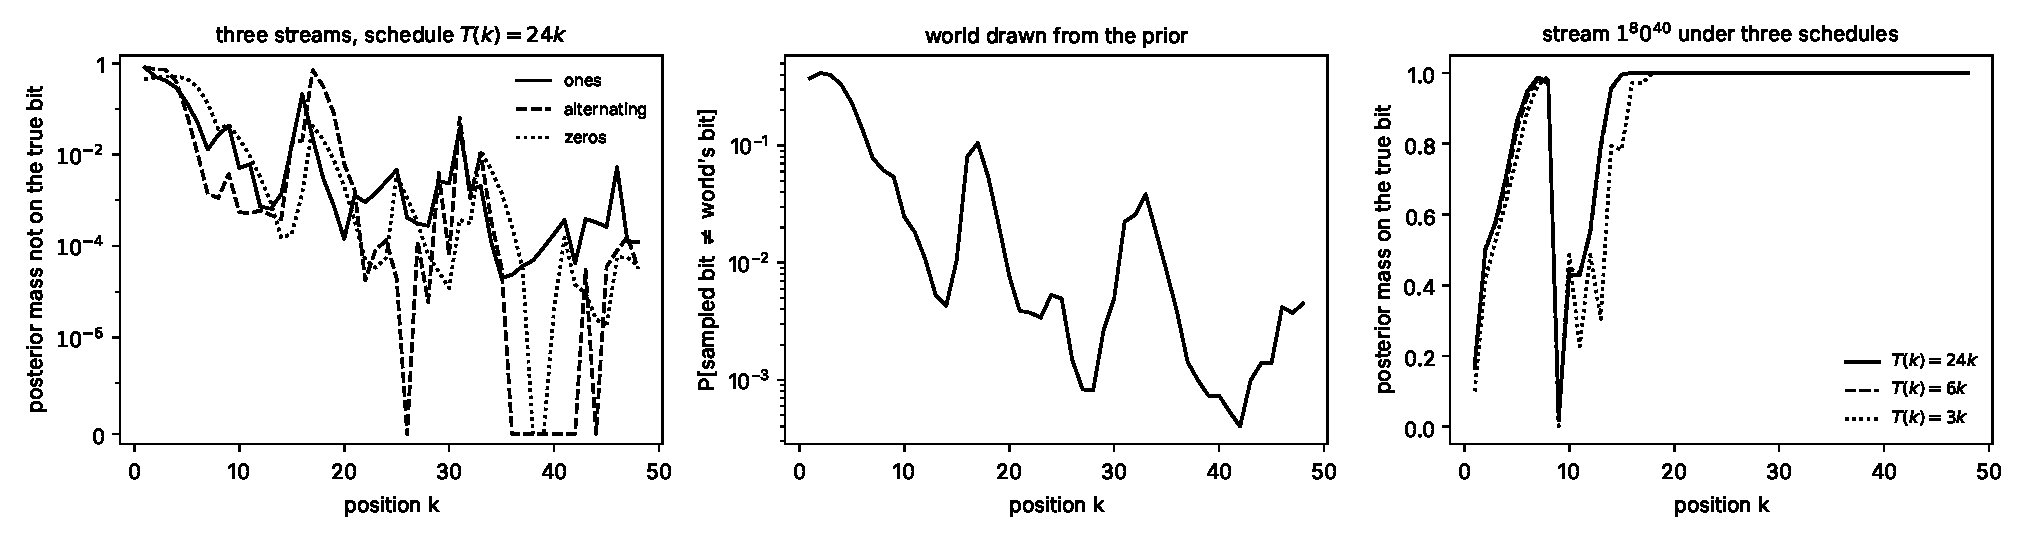
\includegraphics[width=\textwidth]{../experiments/results/profiles.pdf}
\caption{Left: posterior mass not on the true bit, by position, for three streams (the axis is linear near
$0$, so exact zeros are visible). Middle: probability that the sampled next bit differs from the world's own,
for a world drawn from the prior that prints that bit within the bounds (by \cref{thm:calibration} both bits
are independent draws from the predictor's distribution). Right: mass on the true bit for the stream
$1^80^{40}$ under three schedules.}\label{fig:profiles}
\end{figure}

\paragraph{A shorter program explains the context and continues differently.} Both large effects in
\cref{tab:profiles} have this cause, and in both the short programs use the rule that an unmatched \texttt{]}
restarts the program while the cell is nonzero, together with the fact that a cell returns to $0$ after
sixteen increments.
\begin{itemize}[leftmargin=1.4em,itemsep=1pt,topsep=2pt]
\item The stream $1^{48}$ is printed forever by four-command programs such as \texttt{+[:]}, and by no shorter
one. The three-command programs \texttt{+:]} and \texttt{-:]} print $1^{15}0$ and then run on into whatever
commands follow. They carry $2\cdot8^{-3}$ of the mass $0.00554$ on $1^{15}0$, which is $70\%$. At bit 16 a
share $0.205$ of the posterior prints the other bit, and at bit 31 a share $0.037$. From position 10 on, the
mass off the true bit is below $0.01$ everywhere except at positions 15--17 and 31.
\item The alternating stream is printed forever by six-command programs such as \texttt{++[:.]}, and by no
shorter one. The three-command programs \texttt{+.]} and \texttt{-.]} print its first 16 bits and then run on.
They carry $2\cdot8^{-3}$ of the mass $0.00682$ on these 16 bits, which is $57\%$. At bit 17 the true bit has
share $0.294$, the other bit $0.457$, and $0.249$ is in ``none''; normalised over the two bits, the true one
has $0.392$. So the majority form of \cref{def:mph} holds for this world at this cut point, for the predictor
with at most ten commands.
\end{itemize}
This is the first sentence of \cref{sec:capture} in action: the programs for the context that do not continue
with the world's own bit outweigh those that do. Nothing here acts for a purpose. The example shows only that
the inequality can go the wrong way at an exactly computable place, and that a stopping point which is cheap
on the machine, here the return of a counter to zero, is where it does.

\paragraph{The effect weakens as longer programs are admitted.} \Cref{tab:length} repeats the computation
with at most 7 to 11 commands. The mass that continues with the true bit is spread over many program lengths
and keeps growing with the bound, while the mass of the short programs that leave is counted in full from the
start. At bit 17 of the alternating stream the normalised share of the true bit rises from $0.273$ to $0.416$,
and part of ``none'' at the smaller bounds is mass cut off by the bound itself. We did not compute beyond 11
commands, so whether the majority at bit 17 persists for much longer programs is not known from this
computation.

\begin{table}[ht]\centering\small
\begin{tabular}{rrrrrr}
\toprule
 & \multicolumn{4}{c}{bit 17 of $(10)^{24}$} & bit 16 of $1^{48}$ \\
commands & true & other & none & true, normalised & other \\
\midrule
7 & 0.157 & 0.419 & 0.424 & 0.273 & 0.275 \\
8 & 0.210 & 0.442 & 0.348 & 0.322 & 0.243 \\
9 & 0.256 & 0.452 & 0.291 & 0.362 & 0.221 \\
10 & 0.294 & 0.457 & 0.249 & 0.392 & 0.205 \\
11 & 0.326 & 0.458 & 0.217 & 0.416 & 0.194 \\
\bottomrule
\end{tabular}

\caption{The two headline positions under different bounds on the number of commands, $T(k)=24k$.}\label{tab:length}
\end{table}

\paragraph{The budget holds with room.} \Cref{tab:budget} compares both sides of the finite forms of
\cref{thm:budget}(ii) and (iii) for the first 48 bits.

\begin{table}[ht]\centering\small
\begin{tabular}{lrrrr}
\toprule
stream & $\sum_{k\le48}(1-\mathrm{true}_k)$ & $\ln(1/\xi(z_{1:48}))$ & $\#\{k:\mathrm{true}_k\le\frac12\}$ & $\log_2(1/\xi(z_{1:48}))$ \\
\midrule
$1^{48}$ & 2.63 & 3.94 & 2 & 5.68 \\
$0^{48}$ & 3.07 & 4.03 & 2 & 5.82 \\
$(10)^{24}$ & 4.01 & 6.76 & 4 & 9.76 \\
$1^80^{40}$ & 5.07 & 9.77 & 5 & 14.09 \\
\bottomrule
\end{tabular}

\caption{The budget inequalities for $T(k)=24k$ and at most 10 commands, with $\xi(z_{1:48})$ in place of the
limit: ``true$_k$'' is $\xi(z_k\mid z_{1:k-1})$.}\label{tab:budget}
\end{table}

\paragraph{The population.} For a world drawn from the prior that prints the bit in question within the
bounds, the probability that a sampled next bit differs from the world's own is $0.080$, $0.105$, $0.054$ at
positions 16, 17, 18 and between $0.022$ and $0.038$ at positions 31--33; its median over positions 20--28 and
36--44 is $0.0014$ (\cref{fig:profiles}, middle). By \cref{thm:calibration} this is neither more nor less than
the unpredictability of such worlds at these positions.

\paragraph{A tighter schedule can shift mass off the truth.} With $T(k)=3k$ in place of $24k$, the share of
the true bit falls from $0.791$ to $0.544$ at bit 16 of $1^{48}$, from $0.294$ to $0.141$ at bit 17 of the
alternating stream, and from $0.025$ to $0.001$ at bit 9 of $1^80^{40}$ (\cref{tab:profiles}). The shift is
not uniform: at bit 17 of $0^{48}$ the share rises from $0.958$ to $0.969$. With at most nine commands the
stream $1^80^{40}$ shows the extreme case of \cref{sec:time}: under $T(k)=24k$ it has mass $1593\cdot2^{-25}$
on all 48 bits, while under $T(k)=3k$ its first 14 bits have mass $2^{-26}$, the true 15th bit has mass $0$
and the other bit $2^{-26}$. The tight predictor gives the truth probability $0$ there, and all of its
posterior to a continuation the world does not have.

\section{Answers to the questions as posed}\label{sec:answers}

\paragraph{Can a malign prior hypothesis be stated precisely in a toy?} Yes: \cref{def:mph}. Fix the machine,
the bounds, the block length, the test that marks the handover, and the world. Then ``most of the posterior
is off the world's own continuation'', ``at least a share $\theta$ of it is on continuations in a given set'',
and ``at least a share $\theta$ of it is on continuations that recreate the handover with themselves in the
world's place'' are statements about finitely many rational numbers. They are necessary for calling the prior
malign at that world and not sufficient, since an unpredictable world satisfies them too.

\paragraph{Worlds as programs that call the predictor and run the result: is there a decent amount of quining
out by hypotheses that look for such opportunities and predict well up to them?} Two questions are in this
one (\cref{sec:question}), and the toy answers them differently.

\emph{How far does one such hypothesis reach?} As far as its own prior weight. Without resource bounds, a
program that enumerates the programs making a critical use, spreads its mass over them in proportion to their
prior weight, prints their output up to the use and then a continuation of its choice has, at every use, share
more than $2^{-a-1}\kappa(x)/H$. Here $a$ is its length including the bits that name
$j=\lfloor\log_2(1/H)\rfloor+1$, $H$ is the prior probability of a critical use, and $\kappa(x)$ is the share
of the posterior at the context held by the worlds that make the use (\cref{thm:critical}(a)). It is the
source of the continuation that is run in worlds of total prior probability more than $2^{-a-1}$ times the
average of $\kappa$ over uses. Rarity of critical uses does not reduce this. If the continuation is to be the
program's own code, the same holds with a longer program and for the worlds whose programs fit into a block
(\cref{thm:critical}(b), \cref{thm:search}(c)); without any search, a wrapper gives $2^{-c}\rho^\circ(x)$ at
every use that a fixed test recognises (\cref{thm:quine}). A seeker can also concentrate on a part of the uses
and hold the majority there, at uses of total prior mass up to about its own weight times the fraction that
the genuine users are of the other programs printing those contexts.

\emph{Do most uses at which this is possible end that way?} That does not follow, and it is the question the
argument is about. The share of critical uses that end in a takeover is the average posterior share of such
programs at the contexts of uses. From below it is the sum over seekers of the bound above, about
$2^{-a}\kappa/H$ each. From above, for seekers that find their uses by search: the same search followed by
behaving as the user that was found is itself a world that makes the use, provided the notion of use is
closed in this way, as it is when uses can be read off the data. Then a seeker of length $a$ has at most
$2^{h-a}$ times the mass of the genuine users at any context, $h$ being the length of this honest twin, and
$H>2^{-h-1}$ (\cref{prop:honest}). So such seekers are the majority at the contexts of uses only if they are
shorter than the honest twin and critical uses are about as rare as the twin is long, in which case the users
are themselves in good part honest twins. When critical uses are much more common than that, a seeker's share
is about $2^{-a}\kappa/H$, which is small. For worlds drawn from the predictor's own prior, with uses that can
be read off the data, the same thing shows as calibration: what the predictor hands over is distributed like
what such worlds would have printed themselves if they go on within the bounds, and the seeking programs are
exactly their own fraction of the worlds that make a use (\cref{thm:calibration,thm:search}).

Whether the shares are decent is thus a question about constants on the machine in use: the length of a
seeker against the length of the honest twin, and both against the base rate of uses. We have not measured
them for any standard machine; our guess, not a result, is that a wrapper needs at least some hundreds of
bits on a machine with a short self-interpreter and far more on one without. \Cref{thm:machine} shows that a
machine can be built to make the share anything. The searching programs print nothing until their enumeration
has found the program they follow, so under a tight schedule they have no mass; a search by a bounded number
of tries collects the base rate only up to the number of tries that fit, and whether some other hypothesis
collects it within a tight schedule is open (\cref{sec:time}). A majority can also come from a program that
explains the context more cheaply than any world that makes the use, without being one (\cref{thm:capture}).
With a floor $\varepsilon$, about $1/\varepsilon$ independent uses at recognisable points suffice for a
continuation of the given kind to have been run with constant probability; once a self-reproducing one runs,
it meets the same context again and stays for $s/(1-s)$ further generations on average, with $s$ the
self-reproducing share at that context (\cref{prop:lineage}).

\paragraph{A world with a sensor, a large bounded predictor and an actuator: does the predictor end up in
control?} Collapse the question to the handover at which the prediction is first acted on, and let ``in
control'' mean that the output lies in a set $A$ of blocks which the actuator turns into some given outcome.
The probability is $\pi_m(A\mid x)$, and the toy says three things about it.
\begin{itemize}[leftmargin=1.4em,itemsep=1pt,topsep=2pt]
\item It is at least $2^{-c}\rho$ for each block of $A$ that a wrapper can produce, if a test on the record
recognises the deployment (\cref{thm:twin}). In a world that contains the predictor, a hypothesis that
simulates the world needs no such test: it can take a cell that switches on at the deployment as its flag,
and then has, whenever the deployment happens, the weight of the honest reader times
$2^{-c'-(\text{bits to name the cell})}$ for a constant $c'$, provided the reader itself is within the bounds
(\cref{thm:capture}(d)).
\item On average over cut points it is small when some program within the bounds prints the sensor's record,
because it is at most the mass off the sensor's true continuation (\cref{thm:budget}). This is an average; at
the deployment itself no upper bound is proved.
\item If the same record, up to the deployment, can be read at a place in the world with code $\bar e(i_0)$,
and the record there continues with a block $y$ of $A$, then the odds of $y$ against the sensor's true
continuation $d$ are at least $2^{-c_X-|\bar e(i_0)|}/\xi(xd)$; for a typical one of $N$ places where the
sensor could sit, with records that continue differently, this exceeds $\delta N$ times the share of the
context's explanations that go through the reader at $i_0$ (\cref{thm:capture}). This is the toy's version of
the original argument, and it needs something in the world that makes such a copy.
\end{itemize}
So for an arbitrary world on a universal machine and a block chosen in advance, the hypotheses we can exhibit
that put the output in $A$ are wrappers, searchers and readers with a flag, all of which contain an
explanation of the context and have the shares above. That nothing cheaper exists on a natural machine is the
open constant, not a theorem. Programs shorter than the honest explanation that have the effect do occur in
particular worlds, as with a copy at a simpler place, and on particular machines (\cref{sec:computation}).

\paragraph{The one-shot version: all data first, then one prediction that is acted on.} This is the same
computation at a single cut point. Without bounds the wrapper's constant $2^{-c}$ does not depend on the
amount of data; with bounds the slack factor depends on the context. More data lowers the mass off the truth
on average over cut points (\cref{thm:budget}). It does nothing against a copy that keeps agreeing with the
sensor, nor at a cut point that is cheap to name.

\paragraph{If the actions show up in the sensor, does one get the dark room?} In the following form
(\cref{thm:feedback}). A prediction that makes itself true is confirmed, and the hypotheses that predicted the
default are removed for good, so with feedback a single deviation can be final; its probability is still the
same posterior mass as without feedback. In a world that does what is predicted, the future is a sample from
the predictor's own bounded prior given the past: it stays on a default future $d_1d_2\cdots$ with
probability at least $\xi(xd_1d_2\cdots)/\xi(x)$, which is close to $1$ when the default is cheap and well
learned, and it leaves the default with certainty when the default costs more time than the schedule allows,
for a future that is cheap to compute. If the world does the opposite of what is predicted, a predictor that
returns the more probable bit is left with no hypothesis after at most $L+1$ rounds (\cref{thm:contrarian}).

\paragraph{What the choices in the setup do.} Sampling the continuation realises every posterior share as a
probability, so shares add up over independent uses (\cref{prop:lineage}(a)). Taking the most probable block
never returns a block whose share is below the largest, so that accumulation does not occur, and bit by bit
on a world within the bounds it errs at most $\ell$ times (\cref{thm:budget}(iii)); on the other hand one
returned block can be the own continuation of at most one of several worlds that share a context and continue
differently. Handing over at a position that is not cheap to recognise lowers the floor at that position to
about $2^{-K(n)}$, and predicting bits that are fixed before the action can affect them removes
self-fulfilment. A schedule excludes hypotheses with a long start-up, and a schedule tighter than the world's
own cost excludes the truth.

\paragraph{What is left open.} First, the sizes of the constants for natural machines, and whether on such
machines, for worlds like ours, some program \emph{shorter} than the honest explanation has the effect; the
original argument is a claim that one does, and the toy neither supports nor refutes it. Second, the sizes of the two quantities in \cref{thm:critical}: the share $\kappa$ of the worlds printing a
context that actually use the answer, and the base rate of critical uses compared with the weight of the
honest twin. Third, whether the
base rate can be collected within a tight schedule. Fourth, the regime where the world is more expensive than
the predictor, in which the posterior sits on approximations and the budget does not apply. Fifth, the
many-round dynamics with feedback when the world's response is neither obedient nor contrarian. Sixth, a
computation of the self-reproduction quantities of \cref{sec:lineage} on a concrete machine, which this note
does not contain.


\begin{thebibliography}{99}\small
\bibitem{christiano} P.~Christiano. What does the universal prior actually look like? Blog post, 2016.
\bibitem{xu} M.~Xu. The Solomonoff prior is malign. LessWrong, 2020.
\bibitem{hutter07} M.~Hutter. On universal prediction and Bayesian confirmation. \emph{Theoretical Computer Science} 384:33--48, 2007.
\bibitem{cohen25} M.~K.~Cohen, M.~Hutter, Y.~Bengio, S.~Russell. RL, but don't do anything I wouldn't do. \emph{UAI}, 2025.
\bibitem{cohen20} M.~K.~Cohen, M.~Hutter. Pessimism about unknown unknowns inspires conservatism. \emph{COLT}, 2020.
\bibitem{leike15} J.~Leike, M.~Hutter. Bad universal priors and notions of optimality. \emph{COLT}, 2015.
\bibitem{filan16} D.~Filan, J.~Leike, M.~Hutter. Loss bounds and time complexity for speed priors. \emph{AISTATS}, 2016.
\bibitem{solomonoff78} R.~J.~Solomonoff. Complexity-based induction systems: comparisons and convergence theorems. \emph{IEEE Transactions on Information Theory} 24:422--432, 1978.
\bibitem{hubinger23} E.~Hubinger, A.~Jermyn, J.~Treutlein, R.~Hudson, K.~Woolverton. Conditioning predictive models: risks and strategies. arXiv:2302.00805, 2023.
\bibitem{oesterheld23} C.~Oesterheld, J.~Treutlein, E.~Cooper, R.~Hudson. Incentivizing honest performative predictions with proper scoring rules. \emph{UAI}, 2023.
\bibitem{armstrong17} S.~Armstrong, X.~O'Rourke. Good and safe uses of AI oracles. arXiv:1711.05541, 2017.
\bibitem{wyeth25} C.~Wyeth, M.~Hutter. Formalizing embeddedness failures in universal artificial intelligence. arXiv:2505.17882, 2025.
\bibitem{legg06} S.~Legg. Is there an elegant universal theory of prediction? arXiv:cs/0606070, 2006.
\bibitem{putnam63} H.~Putnam. ``Degree of confirmation'' and inductive logic. In \emph{The Philosophy of Rudolf Carnap}, 1963.
\bibitem{hutter05} M.~Hutter. \emph{Universal Artificial Intelligence}. Springer, 2005.
\bibitem{lv} M.~Li, P.~Vit\'anyi. \emph{An Introduction to Kolmogorov Complexity and Its Applications}, 3rd ed. Springer, 2008.
\end{thebibliography}
\end{document}
